% Paquets généraux
\documentclass[a4paper,12pt,titlepage]{article}
\usepackage[T1]{fontenc}
\usepackage[utf8]{inputenc}
\usepackage[french]{babel}
\usepackage[gen]{eurosym}
%\usepackage[dvips]{graphicx}
\usepackage{fancyhdr}
\usepackage{pdfpages} 
\usepackage{multido}
\usepackage{hyperref}
%\usepackage{textcomp}
%\usepackage{aeguill}
\usepackage{schemabloc}
\usepackage[bitstream-charter]{mathdesign}
\usepackage{pstricks}
\usepackage{helvet}

\newcommand{\id}{54}
\newcommand{\nom}{Liaisons mécaniques}
\newcommand{\sequence}{04}
\newcommand{\num}{01}
\newcommand{\type}{TP}
\newcommand{\descrip}{Modélisation d'un solide. Comportement des liaisons mécaniques. Modéliser les mécanismes du laboratoire par un schéma cinématique, paramétré.}
\newcommand{\competences}{A3-C4: Analyse d'architecture et de comportement \\ &  Mod1-C1: Isolement d'un solide ou d'un système de solides \\ &  Mod2-C10-1: Modèle de solide indéformable \\ &  Mod2-C11: Modélisation géométrique et cinématique des mouvements entre solides indéformables \\ &  Mod2-C12: Modélisation cinématique des liaisons entre solides \\ &  Mod2-C15: Modélisation des actions mécaniques \\ &  Rés-C6: Utilisation d'un solveur ou d'un logiciel multi physique \\ &  Com1-C1: Différents descripteurs introduits dans le programme \\ &  Com2-C4: Outils de communication}
\newcommand{\nbcomp}{9}
\newcommand{\systemes}{Plateforme Stewart}
\newcommand{\systemessansaccent}{Plateforme Stewart}
\newcommand{\ilot}{2}
\newcommand{\ilotstr}{02}
\newcommand{\dossierilot}{\detokenize{Ilot_02 Plateforme Stewart}}
\newcommand{\imageun}{Plateforme}

\newcommand{\urlsysteme}{\href{https://www.costadoat.fr/systeme/57}{Ressources système}}
\newcommand{\matlabsimscape}{\href{https://github.com/Costadoat/Sciences-Ingenieur/raw/master/Systemes/Plateforme Stewart/Plateforme_Stewart_Simscape.zip}{Modèle Simscape}}
\newcommand{\solidworks}{\href{https://github.com/Costadoat/Sciences-Ingenieur/raw/master/Systemes/Plateforme Stewart/Plateforme_Stewart_Solidworks.zip}{Modèle Solidworks}}
\newcommand{\edrawings}{\href{https://github.com/Costadoat/Sciences-Ingenieur/raw/master/Systemes/Plateforme Stewart/Plateforme_Stewart.EASM}{Modèle eDrawings}}
\newcommand{\test}{Stewart_param1}
\newcommand{\testi}{Stewart_param2}
\newcommand{\testii}{Stewart_param3}
\newcommand{\testiii}{Stewart_param4}
\newcommand{\testiiii}{Stewart_euler}

\newcommand{\auteurun}{Renaud Costadoat}
\newcommand{\institute}{Lycée Dorian}


\usepackage{color}
\usepackage{xcolor}
\usepackage{colortbl}
\usepackage{helvet}
\renewcommand{\familydefault}{\sfdefault}
\usepackage{amsfonts}
\usepackage{amsmath}
%\usepackage{xspace}
\usepackage{varioref}
\usepackage{tabularx}
%\usepackage{floatflt}
\usepackage{graphics}
\usepackage{wrapfig}
\usepackage{textcomp}
\usepackage{tikz}
\usepackage{wrapfig}
\usepackage{gensymb}
\usepackage[european]{circuitikz}
\usetikzlibrary{babel}
\usepackage{ifthen}
\usepackage{cancel}
\usepackage{etoolbox}
\usepackage{multirow}
%\usepackage{boxedminipage}
\definecolor{gris25}{gray}{0.75}
\definecolor{bleu}{RGB}{18,33,98}
\definecolor{bleuf}{RGB}{42,94,171}
\definecolor{bleuc}{RGB}{231,239,247}
\definecolor{rougef}{RGB}{185,18,27}
\definecolor{rougec}{RGB}{255,188,204}%255,230,231
\definecolor{vertf}{RGB}{103,126,82}
\definecolor{vertc}{RGB}{220,255,191}
\definecolor{forestgreen}{rgb}{0.13,0.54,0.13}
\definecolor{blcr}{rgb}{0.59,0.69,0.84}
\definecolor{blfr}{rgb}{0.32,0.51,0.75}
\definecolor{orfr}{rgb}{0.90,0.42,0.15}
\definecolor{orcr}{rgb}{0.90,0.65,0.50}
\definecolor{orangef}{rgb}{0.659,0.269,0.072}
\definecolor{orange}{rgb}{0.58,0.35,0.063}
\definecolor{orangec}{rgb}{0.43,0.32,0.25}
\definecolor{rcorrect}{rgb}{0.6,0,0}
\definecolor{sequence}{rgb}{0.75,0.75,0.75}
\definecolor{competences}{rgb}{0.61,0.73,0.35}
\definecolor{grisf}{HTML}{222222}
\definecolor{grisc}{HTML}{636363}
\definecolor{normal}{HTML}{4087c4}
\definecolor{info}{HTML}{5bc0de}
\definecolor{success}{RGB}{92,184,92}
\definecolor{warning}{RGB}{240,173,78}
\definecolor{danger}{RGB}{217,83,79}
\hypersetup{                    % parametrage des hyperliens
    colorlinks=true,                % colorise les liens
    breaklinks=true,                % permet les retours à la ligne pour les liens trop longs
    urlcolor= blfr,                 % couleur des hyperliens
    linkcolor= orange,                % couleur des liens internes aux documents (index, figures, tableaux, equations,...)
    citecolor= forestgreen                % couleur des liens vers les references bibliographiques
    }

% Mise en page
\pagestyle{fancy}

\setlength{\hoffset}{-18pt}

\setlength{\oddsidemargin}{0pt} 	% Marge gauche sur pages impaire2s
\setlength{\evensidemargin}{0pt} 	% Marge gauche sur pages paires
\setlength{\marginparwidth}{00pt} 	% Largeur de note dans la marge
\setlength{\headwidth}{481pt} 	 	% Largeur de la zone de tête (17cm)
\setlength{\textwidth}{481pt} 	 	% Largeu\textbf{r de la zone de texte (17cm)
\setlength{\voffset}{-18pt} 		% Bon pour DOS
\setlength{\marginparsep}{7pt}	 	% Séparation de la marge
\setlength{\topmargin}{-30pt} 		% Pas de marge en haut
\setlength{\headheight}{55pt} 		% Haut de page
\setlength{\headsep}{20pt} 		% Entre le haut de page et le texte
\setlength{\footskip}{30pt} 		% Bas de\textbf{ page + séparation
\setlength{\textheight}{700pt} 		% Hauteur de l'icone zone de texte (25cm)
\setlength\fboxrule{1 pt}
\renewcommand{\baselinestretch}{1}
\setcounter{tocdepth}{1}
\newcommand{\cadre}[2]
{\fbox{
  \begin{minipage}{#1\linewidth}
   \begin{center}
    #2\\
   \end{center}
  \end{minipage}
 }
}

\newcommand{\reponse}[1][4]
{
\multido{}{#1}
{\begin{center}\makebox[0.9\linewidth]{}  \\
\begin{center}\makebox[0.9\linewidth]{\dotfill} \\ \end{center}
}}

\newcommand{\titre}[1]
{\begin{center}
\cadre{0.8}{\huge #1} 
\end{center}
}


% En tête et pied de page
\lhead{\nom}
\rhead{
\includegraphics[width=2cm]{../../img/logo}}
\lfoot{Renaud Costadoat}
\cfoot{Page \thepage}

\fancypagestyle{correction}{%
  \fancyhf{}
  \lhead{\colorbox{danger}{\begin{minipage}{0.65\paperwidth} \textcolor{white}{\textbf{Correction}} \end{minipage}} }
  \rhead{
\includegraphics[width=2cm]{../../img/logo}}
  \lfoot{Renaud Costadoat}
  \rfoot{\colorbox{danger}{\begin{minipage}{0.6\paperwidth} \begin{flushright}\textcolor{white}{\textbf{Correction}}\end{flushright} \end{minipage}} }}

\renewcommand{\footrulewidth}{0.4pt}

\usepackage{eso-pic}
\newcommand{\BackgroundPic}{%
\put(0,0){%
\parbox[b][\paperheight]{\paperwidth}{%
\vfill
\begin{center}
\hspace{0.5cm}\vspace{0.5cm}
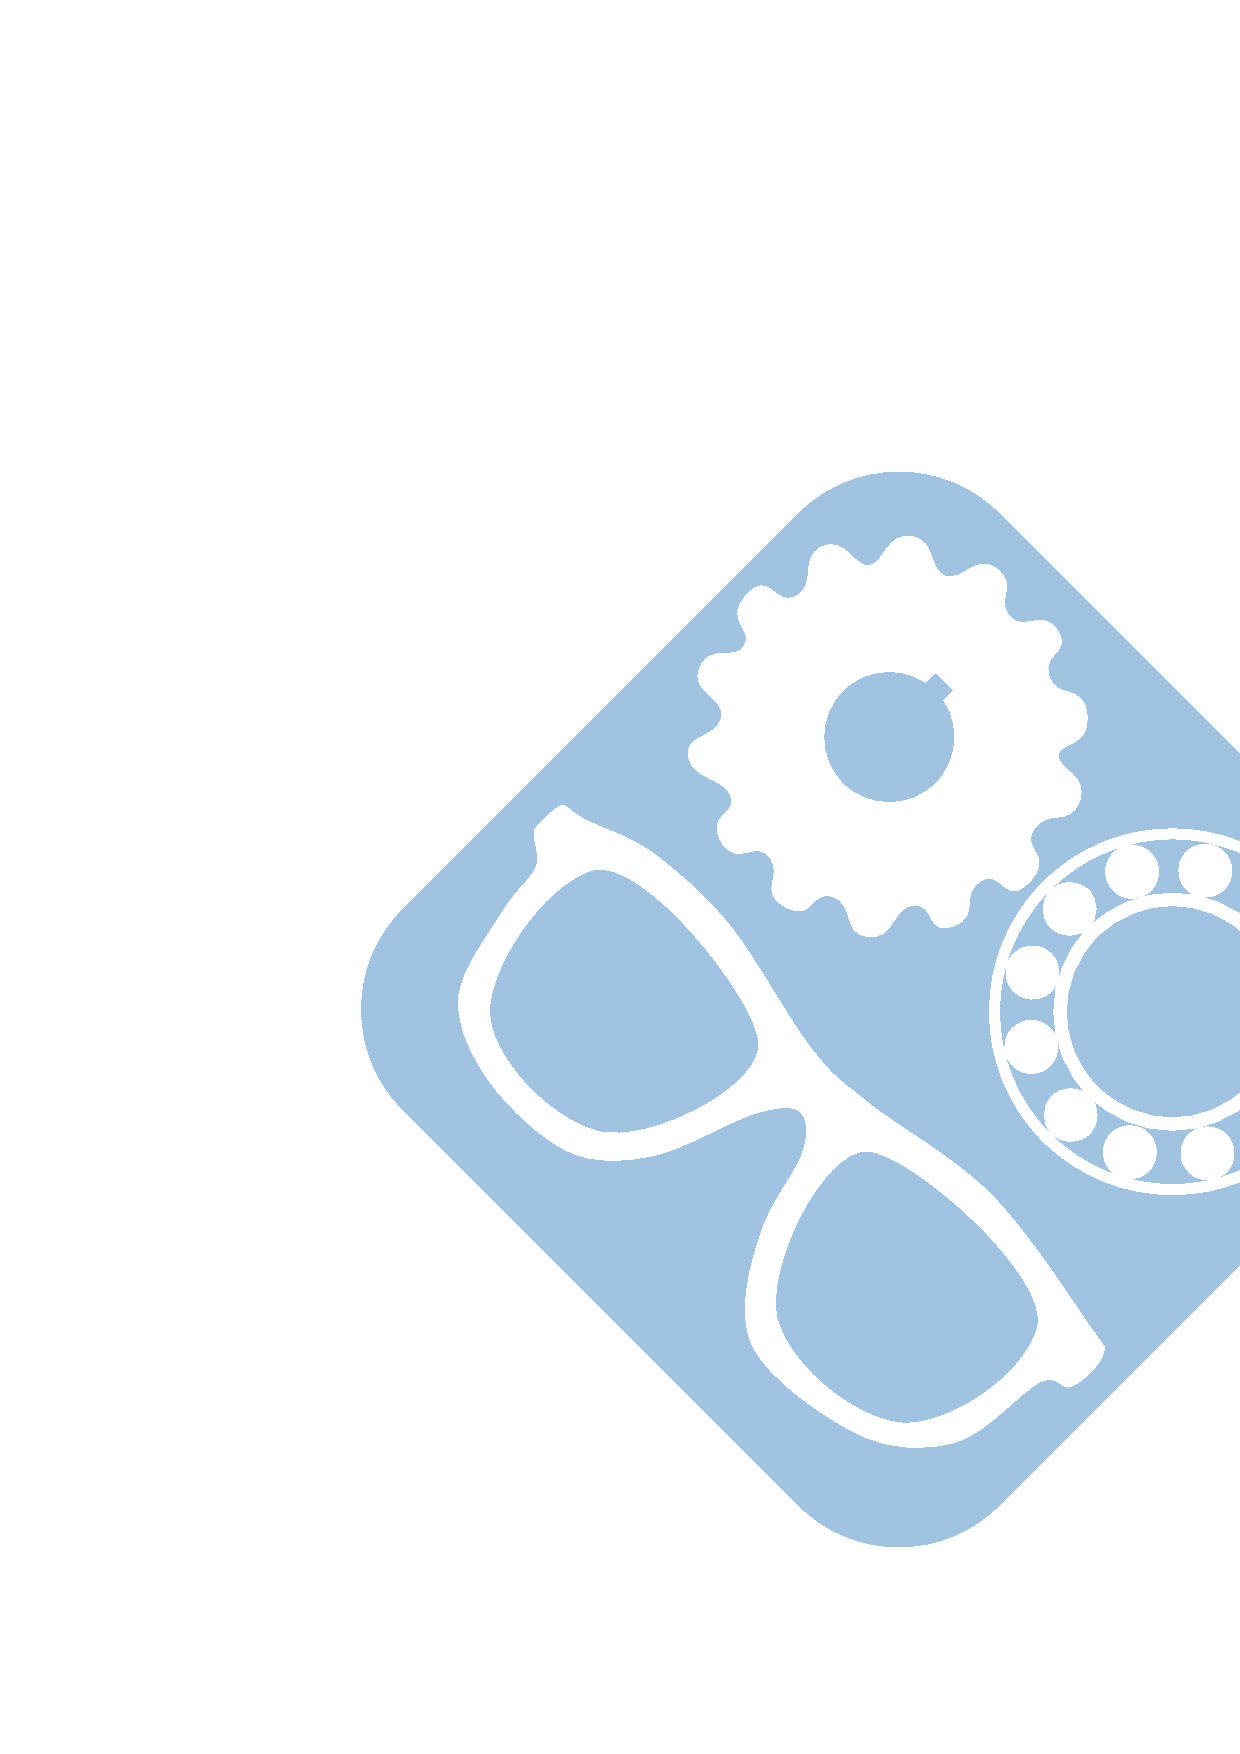
\includegraphics[width=\paperwidth,height=\paperheight,%
keepaspectratio]{../../img/fond3}%
\end{center}
\vfill
}}}

\newcommand{\BackgroundPicdeux}{%
\put(25,-30){%
\parbox[b][\paperheight]{\paperwidth}{%
\vfill
\begin{center}
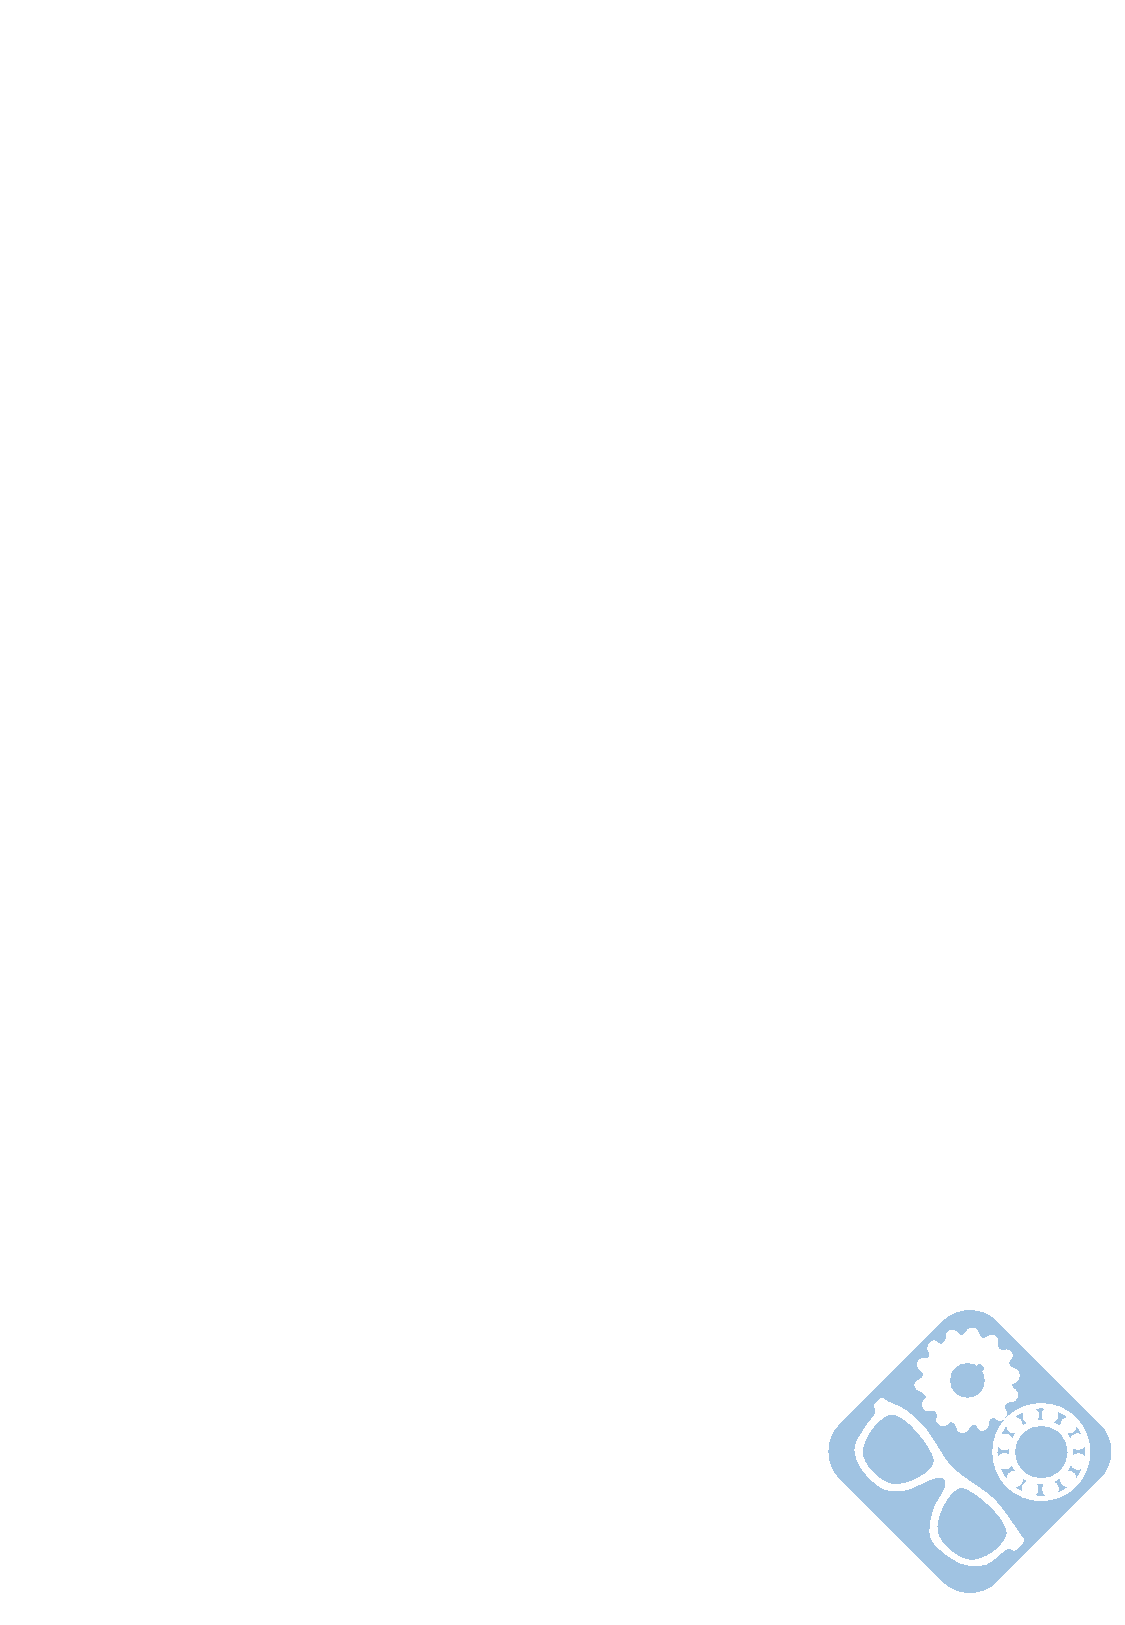
\includegraphics[width=\paperwidth,height=\paperheight,%
keepaspectratio]{../../img/fond4}%
\end{center}
\vfill
}}}

\begin{document}

\AddToShipoutPicture{\BackgroundPicdeux}

\pagestyle{fancy}

\section{Cellule de découpe de vitres}

\begin{figure}[htbp]
\begin{minipage}[c]{.48\linewidth}
\begin{center}
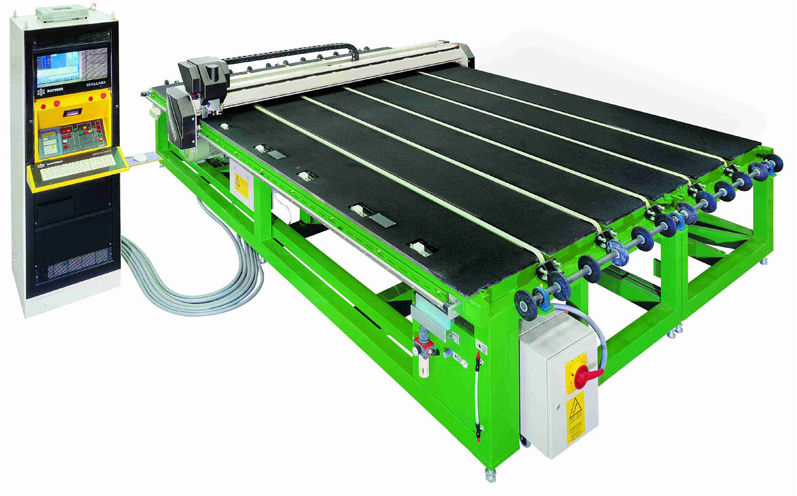
\includegraphics[width=0.8\linewidth]{img/machine_dec_verre.jpg}
\caption{Machine de découpe de verre}
\label{fig:image1}
\end{center}

Un schéma descriptif de la liaison entre l'outil (axe longitudinal) et la table est donné sur la figure \ref{fig:image2}. Une vue en détail est donnée sur la figure \ref{fig:image3}. La liaison globale est donc définie par l'ensemble de ces liaisons élémentaires.

\begin{center}
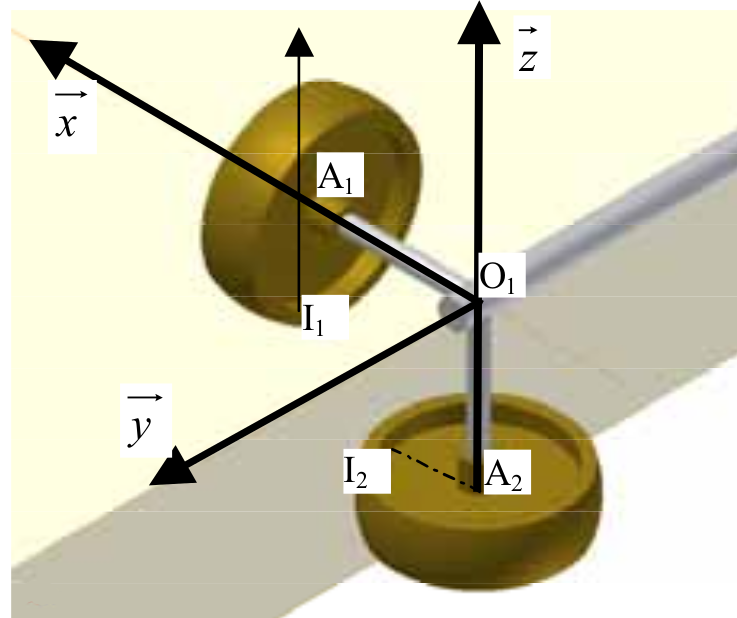
\includegraphics[width=0.5\linewidth]{img/Table2.png}
\caption{Zoom sur la liaison}
\label{fig:image3}
\end{center}
\end{minipage}
\hfill
\begin{minipage}[c]{.48\linewidth}
L'application concerne l'étude du fonctionnement d'une cellule de découpe de vitres, figure \ref{fig:image1}, pour la confection de doubles vitrages. Les vitres à découper sont placées sur une table de découpe sur laquelle se déplace un outil.

\begin{center}
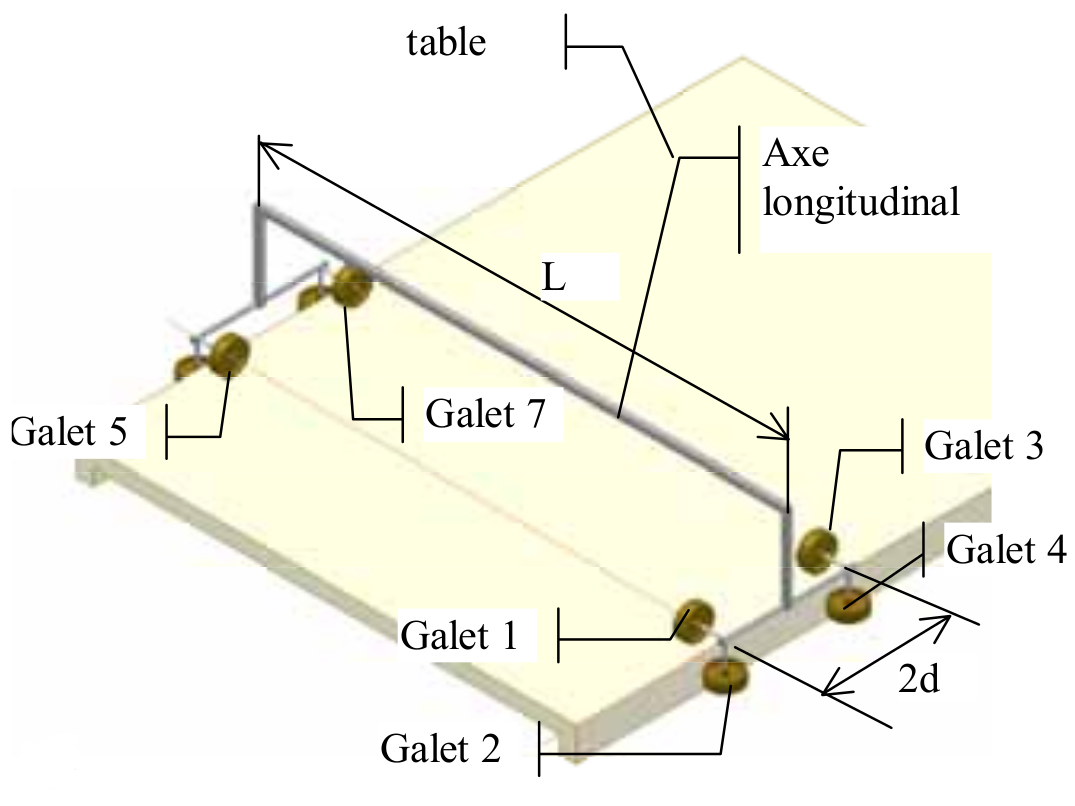
\includegraphics[width=0.8\linewidth]{img/Table1.png}
\caption{Machine de découpe de verre}
\label{fig:image2}
\end{center}

Un système d'axes est placé sur chaque paire de galets, vous utiliserez ce repère pour le paramétrage du mécanisme.
\end{minipage}
\end{figure}

\paragraph{Question 1:}

Réaliser le graphe des liaisons du mécanisme.

\paragraph{Question 2:}

Déterminer la liaison entre le galet 1 et l'axe longitudinal. Et écrire son torseur.

\paragraph{Question 3:}

Déterminer la liaison entre le galet 1 et la table. Et écrire son torseur.

\paragraph{Question 4:}

Déterminer par le calcul la liaison équivalente entre l'axe longitudinal et la table réalisée par l'intermédiaire du galet.

\paragraph{Question 5:}

Déterminer par le calcul la liaison équivalente entre l'axe longitudinal et la table réalisée par les huit galets.

\paragraph{Question 6:}

Déterminer le degré d'hyperstatisme de la liaison.  

\newpage

~\

\cleardoublepage

\section{Etau à serrage manuel}

\begin{figure}[htbp]
\begin{minipage}[c]{.6\linewidth}
Un étau, figure \ref{fig:image4} est un dispositif mécanique qui permet la \og mise en position \fg et le \og maintien en position \fg (serrage) d'une pièce.

Il est composé d'une partie fixe (généralement liée au plan de travail : établi, table de machine-outil), d'une partie mobile, et d'un système de serrage.

C'est souvent par un système vis-écrou que le serrage est effectué : il permet d'appliquer des efforts importants tout en étant irréversible (selon l'angle). Un autre système assez souvent employé est le serrage par excentrique.
\end{minipage}
\hfill
\begin{minipage}[c]{.35\linewidth}
\begin{center}
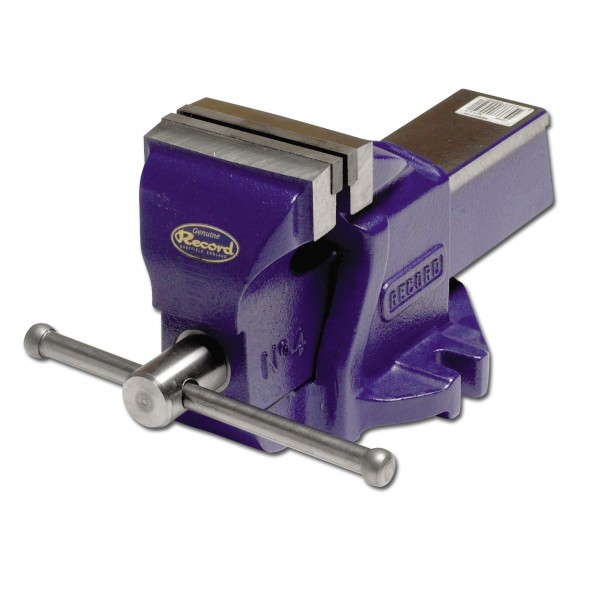
\includegraphics[width=0.8\linewidth]{img/etau.jpg}
\caption{Etau}
\label{fig:image4}
\end{center}
\end{minipage}
\end{figure}

\begin{figure}[htbp]
\begin{minipage}[c]{.3\linewidth}
\begin{center}
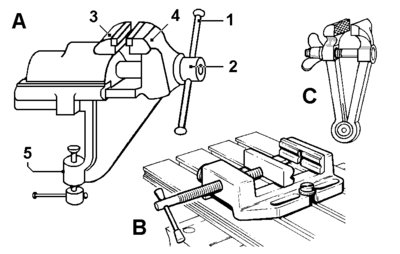
\includegraphics[width=\linewidth]{img/etau_img.png}
\caption{Etau}
\label{fig:image5}
\end{center}
\end{minipage}
\hfill
\begin{minipage}[c]{.69\linewidth}
A : Étau à agrafe.
\begin{enumerate}
 \item Manette de serrage,
 \item Tête de la vis de serrage,
 \item Mâchoire mobile (comportant le mors mobile), guidage complet en translation (un seul degré de liberté) sur 4,
 \item Mâchoire fixe comportant le mors fixe,
 \item Fixation au plan de travail (ici par \og agrafe \fg, avec vis de pression : liaison complète temporaire).
\end{enumerate}
B : Étau de perceuse/fraiseuse

C : Étau manuel (sans fixation sur plan de travail)
\end{minipage}
\end{figure}

Le schéma cinémtique, de la figure \ref{fig:image6}, correspond à ce type de mécanisme.

\begin{figure}[!h]
\begin{center}
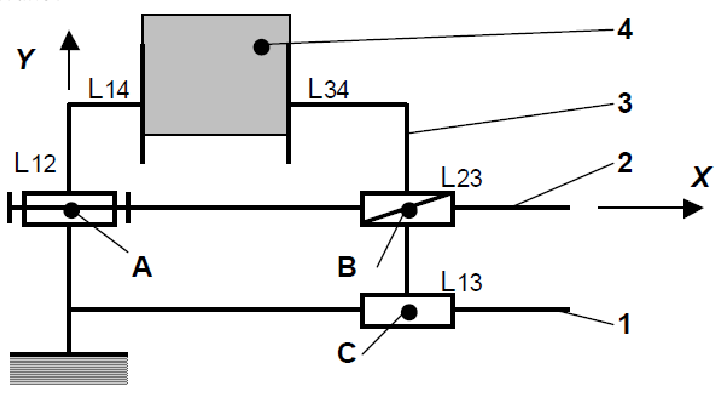
\includegraphics[width=0.5\linewidth]{img/schema_cin_etau.png}
\caption{Schéma cinématique d'un étau}
\label{fig:image6}
\end{center}
\end{figure}

\paragraph{Question 1:}

Réaliser le graphe de liaison du mécanisme.

\paragraph{Question 2:}

Déterminer quelles sont les liaisons mises en place sur ce mécanisme.

\paragraph{Question 3:}

Par un calcul cinématique déterminer le degré hyperstatique et le nombre de mobilités de ce mécanisme.

\cleardoublepage

\section{Joint de cardan}

\begin{figure}[htbp]
\begin{minipage}[c]{.55\linewidth}
Cette solution technique (à ne pas confondre avec la suspension par cardan) est utilisée sur les véhicules pour accoupler deux arbres tournants non alignés, ou dont les positions angulaires, l'un par rapport à l'autre, peuvent varier ; par exemple l'axe du volant et le boîtier de direction, surtout dans le cas d'un volant réglable en hauteur par rapport au conducteur.
\end{minipage}
\hfill
\begin{minipage}[c]{.4\linewidth}
\begin{center}
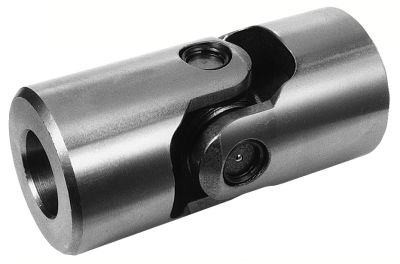
\includegraphics[width=0.7\linewidth]{img/cardan-double.jpg}
\caption{Cardan double}
\label{fig:image7}
\end{center}
\end{minipage}
\end{figure}

\begin{figure}[htbp]
\begin{minipage}[c]{.4\linewidth}
\begin{center}
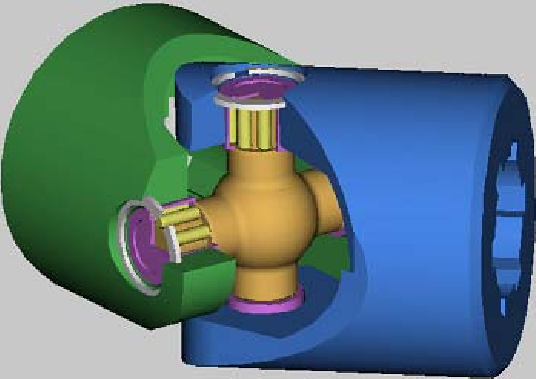
\includegraphics[width=0.7\linewidth]{img/cardan.png}
\caption{Cardan double}
\label{fig:image8}
\end{center}
\end{minipage}
\hfill
\begin{minipage}[c]{.55\linewidth}
Le joint de cardan permet de transmettre le mouvement de rotation d'un arbre d'entrée à un arbre de sortie non parallèles et concourants. Le joint est constitué de deux moyeux liés aux arbres d'entrée et de sortie et d'un croisillon.
\end{minipage}
\end{figure}

\paragraph{Question 1:}

Réaliser un schéma cinématique du mécanisme.

\paragraph{Question 2:}

Tracer le graphe des liaisons du mécanisme constitué d'un bâti, d'un arbre d'entrée, d'un arbre de sortie, et d'un croisillon,

\paragraph{Question 3:}

A partir de calculs cinématiques, évaluer le degré de mobilités en déduire le degré d'hyperstaticité du mécanisme.

\paragraph{Question 4:}

Comment modifier les liaisons pour que le système ne soit pas hyperstatique ?

\newpage

~\

\cleardoublepage

\section{Mécanisme de réglage}

\begin{figure}[htbp]
\begin{minipage}[c]{.45\linewidth}
Cette solution technique est utilisée notament pour certains types de crics qui permettent le levage de véhicules grâce à la rotation d'une manivelle autour d'un axe horizontal.

Ainsi, il transforme la rotation de la pièce 2 en une translation de la pièce 5.
\end{minipage}
\hfill
\begin{minipage}[c]{.50\linewidth}
\begin{center}
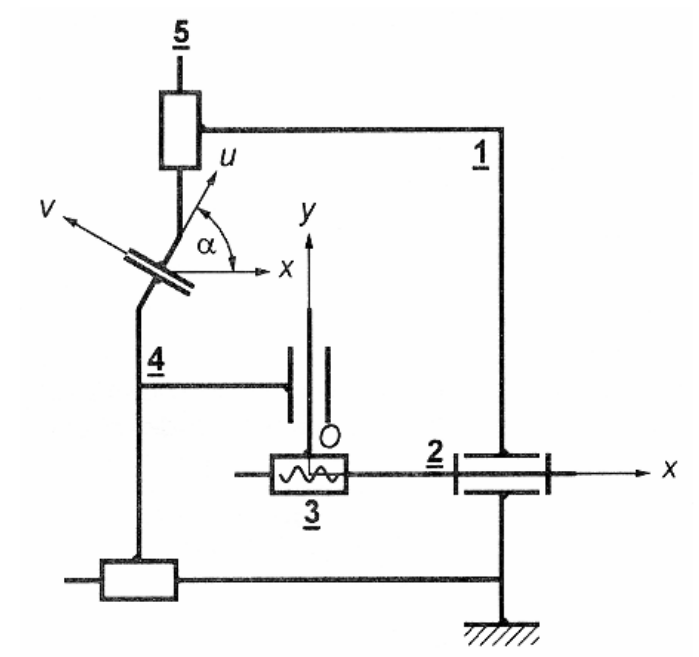
\includegraphics[width=0.8\linewidth]{img/levage.png}
\caption{Système de levage}
\label{fig:image9}
\end{center}
\end{minipage}
\end{figure}

\paragraph{Question 1:}

Tracer le graphe des liaisons du mécanisme.

\paragraph{Question 2:}

A partir de calculs cinématiques, évaluer le degré de mobilités en déduire le degré d'hyperstaticité du mécanisme.

\paragraph{Question 3:}

Comment modifier les liaisons pour que le système ne soit pas hyperstatique ?


\end{document}